%% This is an example first chapter.  You should put chapter/appendix that you
%% write into a separate file, and add a line \include{yourfilename} to
%% main.tex, where `yourfilename.tex' is the name of the chapter/appendix file.
%% You can process specific files by typing their names in at the 
%% \files=
%% prompt when you run the file main.tex through LaTeX.
\chapter{Related Software Tools and Research}
Computational design and digital fabrication are supported through the use of a variety of Computer Aided Design (CAD) software. There are six primary categories of existing software that are relevant to the study of the convergence of these fields: 

\begin{enumerate}
\item{Programing libraries and frameworks for visual computational design.}
\item{Professional CAD tools with computational-design functionality.}
\item{Entry-level programing environments.}
\item{Entry-level CAD tools.}
\item{Novel fabrication and CAD tools.} 
\end{enumerate}

While some tools fall into several of these categories, it is useful to highlight the general functional distinctions and design strategies of each group of tools. 

\section{Programing libraries and frameworks for visual computational design}
Many of the examples of computational design referenced in section \ref{sec:computational_design} were created through the use of custom software tools written in a wide variety of programing languages, libraries and environments. Arguably, computational design can be performed with any programing language that has the capability to output some form of graphic data. In order to facilitate the process, some people have developed programing libraries and toolkits explicitly for computational design. Here I list some of the most prominently used tools in this space and describe their relation to digital fabrication. openFrameworks is a popular open source C++ toolkit developed by Theo Watson and Zach Lieberman that is designed to support a number of creative applications of programming. The toolkit contains wrappers for a variety of commonly used C++ libraries including OpenGL, GLEW, GLUT, libtess2 and cairo for graphics and Assimp for model loading, and facilitates a more immediate use of these libraries in conjunction. Although openFrameworks is frequently used to create interactive screen-based projects, several extensions have been developed which allow for the import and export of .STL model data, making it feasible to use the toolkit to design for digital fabrication \cite{openframeworks}. 

Cinder is another C++ toolkit for computational graphics creation. Cinder was developed by the Barbarian Group, and requires greater programing expertise to use than openFrameworks \cite{cinder}. Similar to OpenFrameworks, Cinder is frequently used to create interactive installations, but it has been used for digital fabrication oriented projects. Nervous Systems used Cinder to develop their Cell Cycle iPad app, which creates cellular bracelets and rings for 3D printing \cite{cell_cycle}. 

Processing is a java-based programing language and development environment created by Casey Reas and Ben Fry. Processing is unique in that it is described as an entry level programing environment but is also an extremely successful professional computational-design tool. Processing contains several libraries that allow it to export to PDF and DXF formats, which enable a translation to digital fabrication \cite{processing}. 

\begin{center}
\begin{figure}[h!]
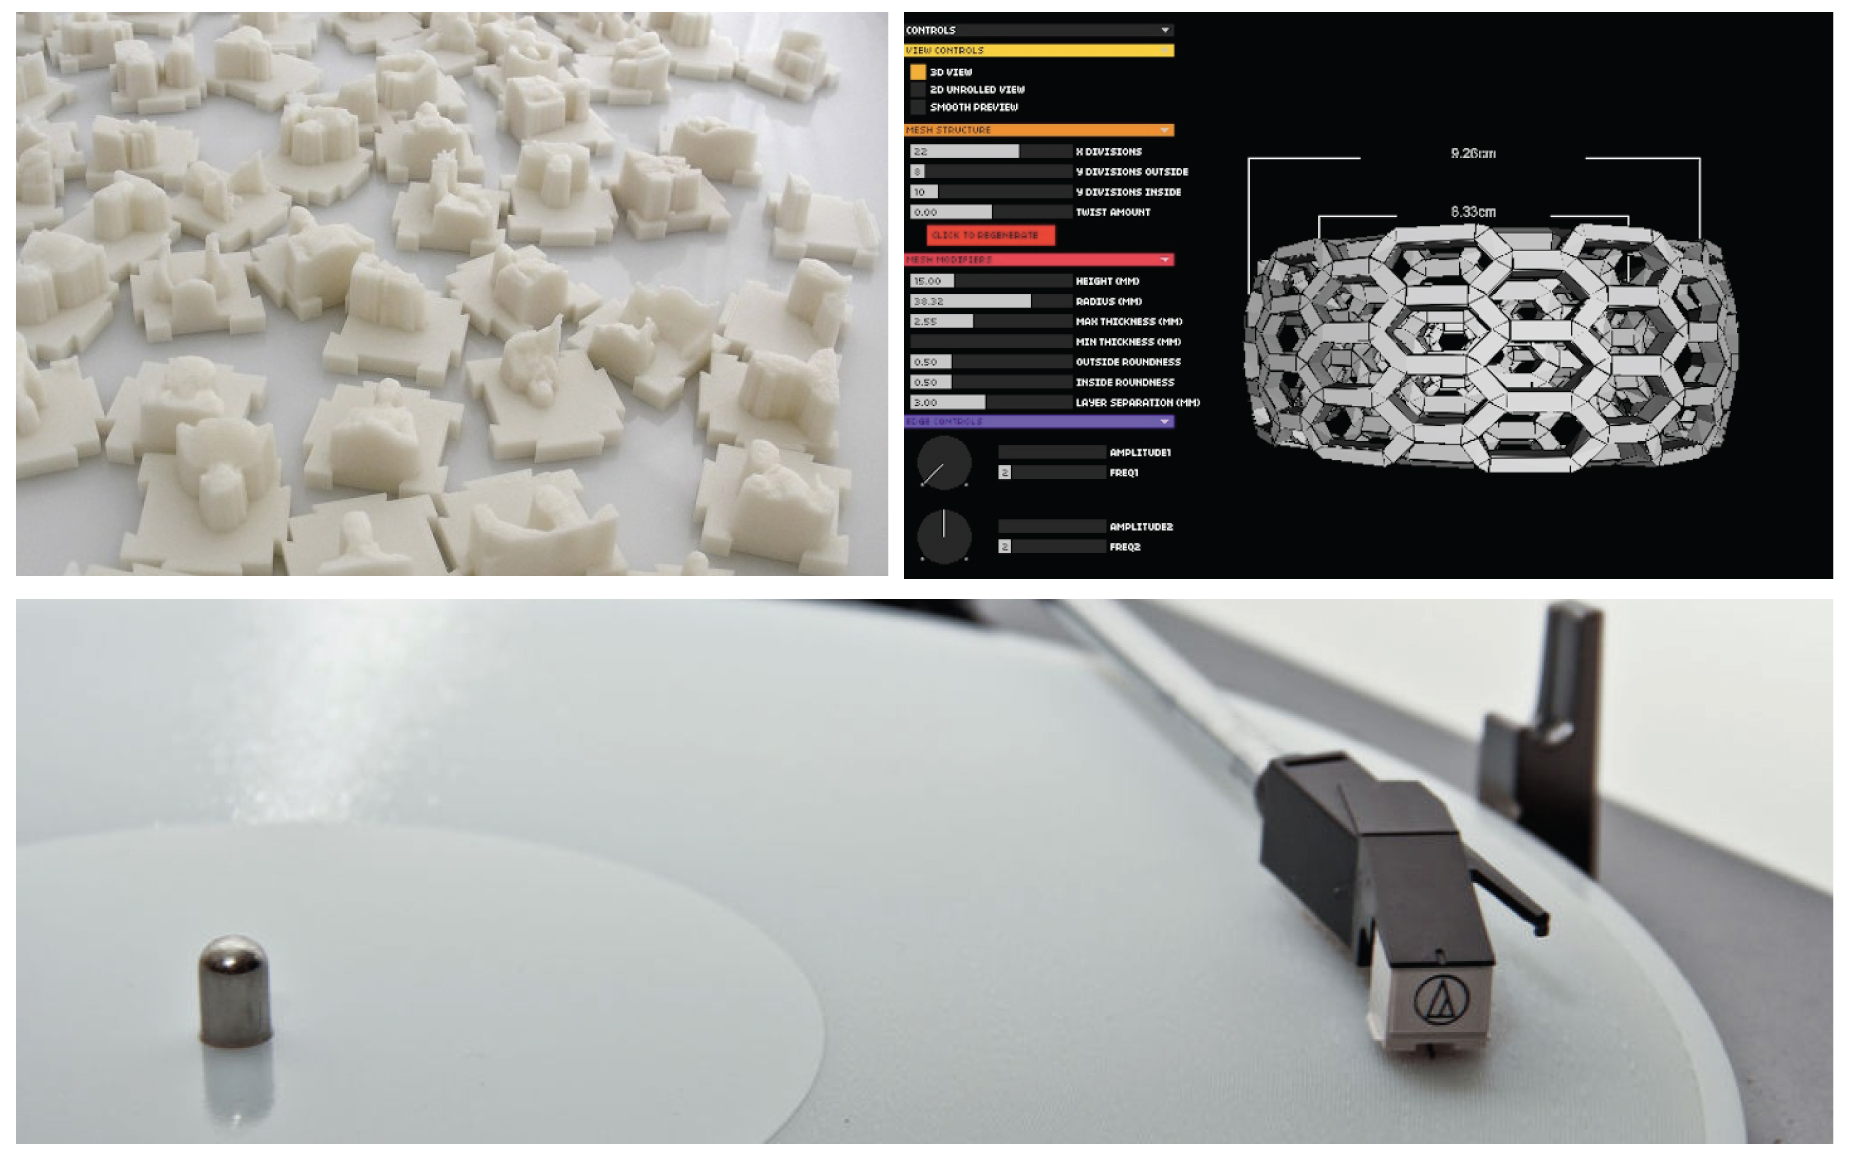
\includegraphics[width=\columnwidth]{images/framework_examples.jpg}
\caption{Clockwise from upper-left: Fabricate Yourself by  Karl D.D. Willis, 3d printed puzzle pieces featuring conference attendees (created with the openFrameworks toolkit, Kinect and a 3d printer), Cell Cycle Bracelet and Ring creation application by Nervous Systems (created with Cinder toolkit), 3d Printed functional record by Amanda Ghassaei, (created using Processing.)}
\label{fig:framework_examples}
\end{figure}
\end{center}

All of these examples use textual programing as the sole means of design. In addition, because openFrameworks and Cinder exist as toolkits, they require the user to write programs in general purpose programing environments such as Visual Studio or Xcode. In the hands of experienced programmers, these tools facilitate remarkable forms of creative expression through code. Because of the difficulty of independently learning textual programing, it is uncommon for people without prior programing experience to use them for computational design without a great deal of instruction and support, let alone apply them to digital fabrication applications. Due to its unique positioning, Processing can act as an exception. We discuss this in greater detail in the section on entry level programing environments.

\section{Professional CAD tools with computational-design functionality}\label{sec:professional_computational_design_tools}
Several forms of professional computational-design tools exist. Many popular graphic-user-interface (GUI) CAD applications include a feature that allows the user to automate certain elements of the program through scripting or programing. For example, in Adobe software like Photoshop and Illustrator, it is possible to write JavaScript-based programs to automate various application procedures. Similarly, 3D modeling tools such as Maya and Blender feature the ability to script behaviors in languages that are syntactically similar to Perl and Python respectively. In all of these examples the programing interface is omitted from the primary interfaces of the application, and must be deliberately activated by the user.

Some professional tools are more explicitly developed for computational design. The most prominent example is Grasshopper, a third-party add-on for the Rhinoceros 3D modeling software. Grasshopper is a data-flow programing environment that lets users combine a variety of modules and blocks to create and adjust 3D models in Rhino. A textual coding module is also available and allows users to integrate C\# scripts using the Rhino API into their program.

DesignScript, a more recent computational design tool, developed by Autodesk, is a domain specific text-based programing environment and language that contains methods to generate and manipulate geometric models that are compatible with existing Autodesk applications. DesignScript is an add-on to the Autodesk AutoCad software and cannot be run independently. DesignScript is intended for use by experienced designers  and 3D modelers who posses a range of programming expertise. The language syntax is based on C\#, however it features the ability to operate in both associative and imperative paradigms, in an effort to support a pedagogical transition between basic and advanced levels of programming \cite{DesignScript}. 

OpenSCAD is a script-based constructive solid geometry modeling tool developed specifically for CAD applications. OpenSCAD contains a custom programing language in which the user can create descriptions of 3d models in a textual format, and display them by compiling the script. This scripting behavior provides the user with pre�cise control over the modeling process and enables the creation of designs that are defined by configurable parameters, however this control comes at the cost of requiring the user to be familiar with textual programing and scripting. OpenSCAD is explicitly developed for experienced programmers and relies on textual input exclusively, In addition, unlike the prior tools mentioned, OpenSCAD is both free and open source, and several variations and derivatives of it exist \cite{OpenScad}.

One of the most important elements of these professional tools is their ability to import and export a wide variety of file formats, thus facilitating the transitions between a digital design and the required file type for a specific fabrication tool. Because to their high-cost and complex feature set, these professional tools are difficult to use without prior experience or extensive practice. With the exception of OpenSCAD, another defining feature of these tools is that they only available as plugins, add-ons  or are developed to supplement an existing graphical tool, rather than serve as the primary method of design. This status of programing as secondary form of interaction poses a practical barrier to novice use of the computational functionality of these tools; the scripting tools in illustrator and photoshop are difficult to locate, Grasshopper must be custom installed along with several dependencies, and only functions on Windows versions of Rhino, and Design Script requires the prior purchase of AutoCAD to operate. While these practical barriers can be overcome, their existence often prevents less experienced users from gaining access. More importantly, the positioning of computational functionality as secondary to the primary method of design points to a larger ideological classification of these forms of design as a specialized and exclusive, rather than serving as a primary method of design. 


 \todo{images of professional level tools}

\section{Entry-level CAD Tools}
A subset of CAD tools have been created that are designed to be more accessible to a wider range of people. These tools provide an option for individuals who lack the experience and access to professional level tools, however they also provide an opportunity for more casual participation in CAD. SketchUp is a 3d modeling tool developed by Google to enable easier forms of 3D modeling. Although SketchUp was not explicitly created to allow people to design for digital fabrication, several independently developed add ons exist that allow users to export designs to file formats that are compatible with a variety of fabrication machine \cite{sketchup}. TinkerCad is another 3d modeling tool designed for entry level users.  As opposed to SketchUp, TinkerCad is explicitly developed to assist in designing for 3d printers and has built in functionality to allow users to export their designs to the .stl format which is compatible with 3D printing \cite{tinkercad}. AutoDesk has also produced several entry level 3d-modeling applications as a part of their 123D series. Many of these applications are designed to interface with digital fabrication, including 123D Make which allows users to convert stock or uploaded 3d models into a series of flat parts which can be fabricated on 2-axis machines like laser cutters, and 123D Creature, which enables users to design a variety of creatures from a set of basic parts and then order a 3d printed model of their finished creature \cite{123D}.  AutoDesk Research has also developed MeshMixer, an application for the intuitive merging and manipulating high resolution triangle meshes. MeshMixer was released to the public and has since become a popular 3d design tool for hobbyist 3D printer users. 

All of the entry level tools listed above vary in their specific approach to creating more accessible forms of CAD. In general they feature a trade off between limited functionality and power, in favor of a simplified tool set and an easier learning curve. Despite these restrictions, it is possible to use these entry level tools to develop highly  complex and sophisticated models \todo{show example image of mesh mixer model}. A more pressing limitation of these tools is their ephemerality. Because entry level CAD tools are often free, and more frequently web based applications, it is common for them to suddenly become unavailable or no longer supported by the company that produces them. Tinkercad serves as a recent example of this wherein the parent company decided to transition to focusing on professional-level CAD tools and as a result, closed down the Tinkercad website and cut off access to the application. TinkerCad was recently acquired by AutoDesk and its website restored, however its future is uncertain.

Several of these entry-level tools also feature some form of scripting or programing functionality. A plugin for Sketchup allows users to automate certain actions by using the Ruby-based SketchUp API. TinkerCad allows users to create Shape Scripts, which are parametric models defined by javascript code. MeshMixer has an C++ API which is not yet publicly available, but is provided to interested parties upon request. While these computational features suggest compelling possibilities, similar to the professional level tools listed above, they are positioned as secondary ways of interacting, and are designed less deliberately than the primary features of the application.

 \todo{images of entry level cad tools and fix citations}

\section{Learning-Oriented programming tools}
Similar to entry level CAD tools, a number of wonderful applications have been created to introduce inexperienced programmers to the realm of computer science. 
Logo, a computational drawing program, serves as the seminal novice programming language founded on principles of constructionism and embodiment \cite{papert}. The Scratch visual programming language is a notable successor to Logo, and allows users to create interactive projects by combining command blocks rather than writing textual code \cite{scratch}. Alice is another programming environment that relies on visual programming, but is targeted towards an older user group than Scratch \cite{alice}. Turtle Art \cite{turtleart} and Design Blocks cite{design blocks} are two visual programming languages inspired by Logo that are designed specifically for visual composition. Processing is a text-based programming environment designed for easy learning, and directed toward artists, designers, and inexperienced programmers \cite{processing}.

Logo, Turtle Art, Design Blocks, and Processing facilitate computational drawing and, therefore, can be viewed as computational-design environments. There remains a gap, however, between novice-oriented programing environments and the novice-oriented CAD tools. In direct contrast to the novice oriented CAD tools described in the preceding section, although learning oriented programing tools can provide an excellent platform for generating digital computational design work, they often lack explicit features for generating and exporting designs that are compatible existing modes of digital fabrication. It is possible to create work-arounds; for example in processing, users can download and install community-created libraries that allow for Stereolithography format (STL), Drawing Interchange Format (DXF), and Portable Document Format (PDF) export. The independent development of export functionality for tools like Processing demonstrates significant interest by the community in combining computational design and digital fabrication. If we wish to open this space for entry level practitioners however, we must design tools that exhibit the tools and techniques for computational design for fabrication as their primary functionality.

\begin{center}
\begin{figure}[h!]
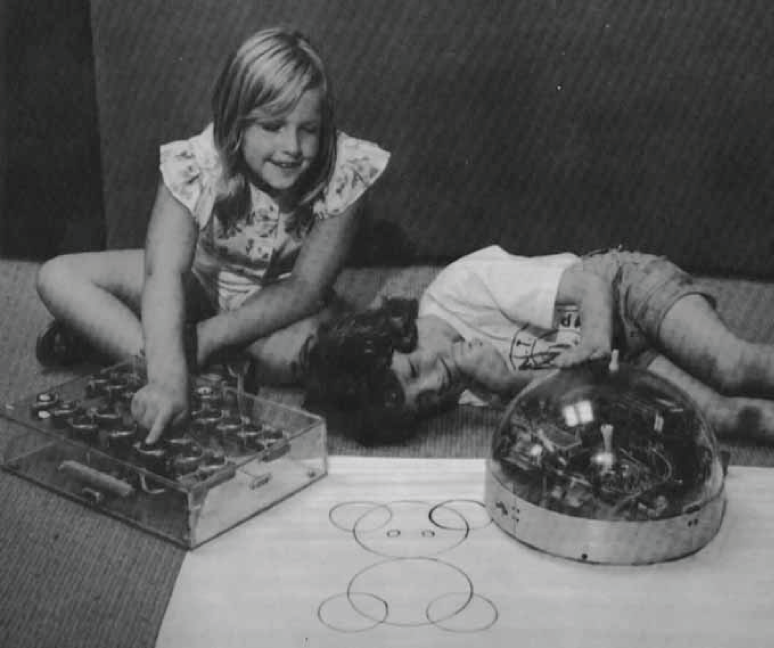
\includegraphics[width=\columnwidth]{images/logo_turtle.png}
\caption{The Logo Turtle robot: an early form of computational design and digital fabrication for novices)}
\label{fig:logo_turtle}
\end{figure}
\end{center}

\section{Novel Fabrication and CAD tools}
In addition to these tools, there are a number of research projects involving novel forms of fabrication and software tools that demonstrate new approaches for computational design and digital fabrication. Sketch It, Make It is a 2D CAD tool that allows users to constrain their designs through gestures made using a digital drawing tablet \cite{sketchit}. Spatial Sketch is a tool that allows users to create abstract 3D sketches via their gestures, and then translates the sketches into a set of slices, which can be fabricated and combined into a finished piece \cite{spatialsketch}.  SketchChair allows users to design their own chair by sketching with a computer stylus \cite{sketchchair}. The resultant design can then be cut on a computer-numerical controlled (CNC) milling machine and assembled into a 3D object. SketchChair includes a simulation tool that allows users to test the usability of their chairs before they cut them. FlatCAD seeks to connect programming and digital fabrication and allows users to build customized construction kits with a laser cutter by programming in FlatLang, a novice-oriented programing language modeled on Logo \cite{flatcad}. Spirogator is a processing based tool that allows users to digitally customize a set of hypotrochoid geared-drawing tools and then view a simulation of those tools in action. The user then has the option of either exporting the resulting design generated by the digital gears and fabricating it directly, or exporting the file paths for the gears themselves, and fabricating them on a laser cutter, to be used as physical drawing tools \cite{spirogator}. 

These examples share several important elements. They are restricted to a relatively narrow domain, but still support a wide range of design variations and personal expression. They contain intuitive and familiar methods of interaction often in the form of drawing and moving sliders. They contain explicit features for making the process of digital fabrication easier for new practitioners, and reduce the possibility of creating designs that will be infeasible to fabricate or are physically unstable. Spirogator and Sketch Chair's simulation tools are particularly interesting in this regard, as they assist the user in predicting some of the behavior of the resultant physical artifact prior to its fabrication. These qualities of domain-specificity, design flexibility, intuitive interaction and practical support for fabrication are important properties for any novice-oriented design software.

 \todo{images of novel cad tools}

%\todo{
%/Garment-Creation CAD and Fabrication tools
%Sensitive Couture
%parsing patterns into 3d garments
%Sketch Based Garment Design
%Art quilt?
%}